Abbildung \ref{fig:Versuchsaufbau} zeigt den schematischen Aufbau der verwendeten Versuchsanordnung. Als Strahlungsquelle wird XXXX\todo{Hier fehlt das Element.}, ein Beta-Strahler verwendet. Der Zähler zählt die Pulse pro \SI{10}{\second}.
\begin{figure}[h!]
	\centering
	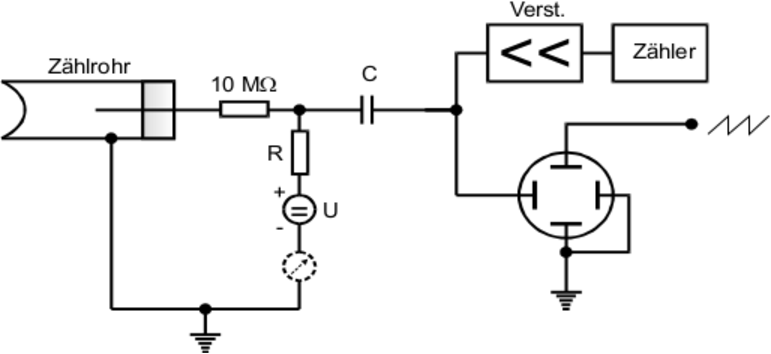
\includegraphics[width=0.7\textwidth]{Versuchsaufbau.pdf}
	\caption{Versuchsaufbau}
	\label{fig:Versuchsaufbau}
\end{figure} \\
\subsubsection*{Messung}\todo{Hier müssen überall noch genaue Werte eingefügt werden.}
Zunächst wird die \textbf{Charakteristik} des Zählrohrs in einem Bereich von $0-700$V aufgenommen. Die Intensität der Strahlung sollte dafür nicht zu hoch sein, da sonst wesentliche Totzeitkorrekturen gemacht werden müssten. \\
Zur Bestimmung der \textbf{Nachentladung} wird ein Oszilloskop verwendet, das die Strompulse über der Zeit anzeigt. Im Zählrohr wird eine Spannung $U~\SI{350}{\volt}$ eingestellt, sodass kaum Nachentladungen auftreten. Die Strahlungsintensität wird dann soweit verringert, dass nur ein einziger von einem $\beta$-Teilchen stammender Puls zu sehen ist. Die Spannung wird dann auf etwa $\SI{700}{\volt}$ erhöht. Nun können die Nachentladungen am Oszilloskop, als weitere Impulse gesehen werden. Die Differenz zwischen Teilchen-Peak und Nachentladungs-Peak wird abgelesen. \\
Die \textbf{Totzeit} kann ganz ähnlich bestimmt werden. Die Intensität wird so groß wie möglich gewählt. Die Differenz zwischen Beginn des Teilchen-Peaks und Beginn des Nachentladungs-Peaks wird abgelesen. \\
Zusätzlich wird die \textbf{Totzeit} mit Hilfe einer zweiten Quelle gemessen. Es wird dazu zunächst die Pulse, die eine Quelle abgibt. Dann die Pulse, die zwei Quellen zusammen emittieren und dann die zweite einzeln. Da die Summe der beiden einzelnen Messungen größer ist, als die der gemeinsamen Messung muss die Totzeit eine relevante Rolle spielen. \\
Zuletzt wird die \textbf{freigesetzte Ladung pro Teilchen} gemessen. Hierfür werden wieder Impulse in einem Zeitintervall gezählt und zudem wird der dabei fließende Strom auf dem Ampère-Meter abgelesen.